\documentclass[11pt,a4paper]{article}

% === Packages ===
\usepackage[utf8]{inputenc}
\usepackage[T1]{fontenc}
\usepackage{amsmath,amssymb}
\usepackage{graphicx}
\usepackage{booktabs}
\usepackage{hyperref}
\usepackage[margin=1in]{geometry}
\usepackage{xcolor}
\usepackage{enumitem}
\usepackage{natbib}
\usepackage{caption}
\usepackage{subcaption}
\usepackage{float}
\usepackage{array}
\usepackage{algorithm}
\usepackage{algpseudocode}
\usepackage{tikz}
\usetikzlibrary{shapes.geometric,arrows.meta,positioning,fit,calc,patterns}
\usepackage{multirow}
\usepackage{pgfplots}
\pgfplotsset{compat=1.18}
\usepackage{listings}

\newcolumntype{L}[1]{>{\raggedright\arraybackslash}p{#1}}

% === Listing style for context block example ===
\lstset{
  basicstyle=\ttfamily\scriptsize,
  frame=single,
  breaklines=true,
  columns=fullflexible,
  aboveskip=6pt,
  belowskip=6pt
}

% === Hyperlink styling ===
\hypersetup{
  colorlinks=true,
  linkcolor=blue!70!black,
  citecolor=blue!70!black,
  urlcolor=blue!70!black
}

% === Title ===
\title{\textbf{Typed Context Blocks for Domain-Constrained Retrieval\\over Structured Knowledge Bases}}

\author{
  Raj Navakoti \\
  \texttt{rajnavakoti@gmail.com}
}

\date{June 2026}

\begin{document}

\maketitle

% =============================================================================
% ABSTRACT
% =============================================================================
\begin{abstract}
Retrieval-augmented generation (RAG) systems typically treat knowledge bases as flat document collections, ignoring structural metadata about entity types, knowledge layers, and typed relationships. We present \textbf{Domain-Constrained Retrieval (DCR)}, a seven-stage retrieval pipeline designed for typed, layered knowledge bases built using the Demand-Driven Context (DDC) methodology. DCR introduces intent-aware query classification, typed graph traversal, confidence-weighted scoring, multi-layer deduplication, and \textbf{gap detection}---a novel mechanism that converts retrieval dead-ends into structured curation signals. We evaluate DCR against two baselines (naive vector search and vanilla RAG) on a synthetic healthcare claims knowledge base containing 410 entities across 15 types and 6 layers, using 50 evaluation questions across 3 independent trials per condition (1,350 total evaluations). DCR achieves 76.0\% CLEAN answers compared to 59.3\% for vanilla RAG (+16.7 percentage points, $\chi^2 = 8.78$, $p = 0.003$) with near-perfect cross-trial consistency (96\% per-question stability). A surprising baseline result---naive vector search (69.3\% CLEAN) outperforming vanilla RAG (59.3\%)---reveals that the \emph{typed ontology} underlying the knowledge base is the primary quality driver, not the retrieval pipeline. Stage-by-stage ablation confirms this: no individual pipeline stage produces a statistically significant quality change, though graph traversal shows a consistent positive effect. Gap detection fires on 80\% of questions, producing 62 structured curation signals per evaluation, independent of answer quality. We discuss the \emph{synthesis bottleneck}---the finding that context content richness dominates retrieval strategy as a determinant of answer quality---and its implications for RAG system design.
\end{abstract}

\noindent\textbf{Keywords:} retrieval-augmented generation, typed knowledge bases, gap detection, domain-constrained retrieval, knowledge curation, entity-relationship retrieval

\vspace{1em}

% =============================================================================
% 1. INTRODUCTION
% =============================================================================
\section{Introduction}
\label{sec:introduction}

Retrieval-augmented generation has become the dominant approach for grounding large language models in domain-specific knowledge~\citep{lewis2020rag}. The standard RAG pipeline embeds documents as vectors, retrieves the top-$k$ most similar chunks to a query, and passes them as context to a generative model. This approach works well when the knowledge base is a flat collection of documents with uniform structure.

Enterprise knowledge bases are rarely flat. In domains such as healthcare claims processing, financial operations, and supply chain management, knowledge is inherently \emph{typed}: systems differ from processes, APIs differ from data models, business terminology differs from technical jargon. These entities exist in typed relationships---a system implements a capability, a process triggers events, a team owns a service---and are organized into semantic layers ranging from structural definitions to behavioral workflows to organizational ownership.

When a standard RAG pipeline encounters such a knowledge base, it has no mechanism to exploit this structure. Vector similarity treats a system entity and a jargon definition identically. There is no way to traverse typed relationships to discover relevant context that is semantically distant but structurally connected. Most critically, there is no way to detect what the retrieval \emph{missed}: if a question requires knowledge about a process that coordinates two systems, and the knowledge base documents the systems but not the coordination process, the pipeline returns the system entities and produces a plausible-sounding but incomplete answer. The failure is silent.

We present \textbf{Domain-Constrained Retrieval (DCR)}, a seven-stage retrieval pipeline designed for typed, layered knowledge bases constructed through the Demand-Driven Context (DDC) methodology~\citep{navakoti2026ddc}. DCR addresses three problems that standard RAG ignores:

\begin{enumerate}[nosep]
  \item \textbf{Type-aware retrieval.} DCR classifies query intent to determine which entity types and knowledge layers are most relevant, uses typed graph traversal to follow relationship edges, and applies layer-priority boosting during score fusion.
  \item \textbf{Context quality.} Confidence-weighted scoring adjusts entity relevance based on curation quality, and multi-layer deduplication ensures diverse, non-redundant context.
  \item \textbf{Gap detection.} DCR's novel contribution: converting retrieval dead-ends---orphan entities with no relationships, ambiguous type assignments---into structured signals that tell knowledge base curators what to improve.
\end{enumerate}

We evaluate DCR on a synthetic healthcare claims knowledge base containing 410 entities across 15 types and 6 knowledge layers. Our experimental design uses 50 evaluation questions, 9 retrieval conditions (3 baselines + 6 ablation), and 3 independent trials per condition (1,350 total evaluations). We report four main findings:

\begin{enumerate}[nosep]
  \item DCR achieves 76.0\% CLEAN answers compared to 59.3\% for vanilla RAG ($+16.7$pp, $p = 0.003$) and achieves the highest per-question stability (96\%) of any condition tested.
  \item Naive vector search (69.3\% CLEAN) outperforms vanilla RAG (59.3\%), revealing that the \emph{typed ontology}---entity types, layers, curated descriptions, and relationships---is the primary quality driver. Score averaging in vanilla RAG introduces noise that degrades performance below simple cosine retrieval on rich typed content.
  \item No individual pipeline stage produces a statistically significant quality change in ablation. The typed retrieval stages collectively improve quality, but on a dense 410-entity knowledge base, none is individually decisive.
  \item Gap detection fires on 80\% of questions regardless of answer quality, producing 62 structured curation signals per evaluation---an observability mechanism for knowledge base health, not a retrieval confidence signal.
\end{enumerate}

The remainder of this paper is organized as follows. Section~\ref{sec:related} surveys related work. Section~\ref{sec:background} describes the typed knowledge base meta-model. Section~\ref{sec:pipeline} details the DCR pipeline architecture. Section~\ref{sec:setup} presents the experimental setup. Section~\ref{sec:results} reports baseline results. Section~\ref{sec:ablation} analyzes stage contributions. Section~\ref{sec:gaps} examines gap detection. Section~\ref{sec:discussion} discusses implications including the synthesis bottleneck. Section~\ref{sec:limitations} addresses limitations, and Section~\ref{sec:conclusion} concludes.

% =============================================================================
% 2. RELATED WORK
% =============================================================================
\section{Related Work}
\label{sec:related}

\subsection{Retrieval-Augmented Generation}

RAG systems augment language model generation with retrieved context to improve factual grounding~\citep{lewis2020rag}. Early systems use dense retrieval with a single vector index. More recent work introduces hybrid retrieval combining dense and sparse methods~\citep{chen2024bge}, multi-step retrieval with query decomposition~\citep{press2023selfask}, and self-reflective retrieval where the model decides whether to retrieve~\citep{asai2024selfrag}. These advances improve retrieval quality on unstructured document collections but do not exploit typed entity structure.

\subsection{Graph-Enhanced RAG}

GraphRAG~\citep{edge2024graphrag} constructs community summaries over a knowledge graph and uses them for query-focused summarization, showing particular strength on global sensemaking queries. GRAG~\citep{hu2024grag} integrates subgraph retrieval into the RAG pipeline, retrieving relevant subgraphs rather than individual documents. HybridRAG~\citep{sarmah2024hybridrag} combines knowledge graph and vector retrieval for information extraction. These approaches demonstrate that structural information improves retrieval, but they operate on general-purpose knowledge graphs rather than typed, layered entity models with an explicit ontology. DCR differs in that it exploits a predefined type system and layer hierarchy rather than inferring structure from text.

\subsection{Knowledge Graphs and Structured Retrieval}

Knowledge graph embedding methods such as TransE~\citep{bordes2013transe} learn entity and relationship representations for link prediction and knowledge base completion. These methods address knowledge base construction and reasoning rather than retrieval for generative contexts. DCR uses the knowledge graph for traversal-based retrieval (typed breadth-first search) rather than embedding-based reasoning.

\subsection{RAG Evaluation}

LLM-as-judge evaluation~\citep{zheng2023judging} has become standard for assessing generated text quality. Recent work highlights judge consistency as a concern: \citet{liu2025consjudge} propose consistency-aware evaluation, and \citet{shankar2024validates} study alignment between LLM judges and human preferences. Our evaluation uses LLM self-scoring with cross-model validation (GPT-4o as independent judge) and multi-trial stability analysis to characterize scoring variance. The SQuAD 2.0 framework~\citep{rajpurkar2018squad} introduced the concept of unanswerable questions; our MISSING category captures the analogous case for knowledge-base-grounded retrieval.

\subsection{Demand-Driven Context}

The DDC methodology~\citep{navakoti2026ddc} provides the upstream knowledge curation framework that produces the typed, layered knowledge bases DCR is designed to query. DDC constructs knowledge bases incrementally through cycles of agent failure analysis: when an AI agent fails to answer a domain question, a human expert curates the missing knowledge into structured entities. This demand-driven process ensures that the knowledge base grows toward the questions actually asked, rather than toward what documentation authors anticipate. DCR extends this loop by providing automated gap detection signals that can trigger new DDC curation cycles.

% =============================================================================
% 3. BACKGROUND: TYPED KNOWLEDGE BASES
% =============================================================================
\section{Background: Typed Knowledge Bases}
\label{sec:background}

DCR operates on knowledge bases structured according to a typed, layered meta-model (Figure~\ref{fig:ontology}). The meta-model defines 18 entity types across 6 semantic layers; a given knowledge base instantiates a subset of these types. The layers partition domain knowledge by the category of question each answers:

\begin{itemize}[nosep]
  \item \textbf{Structural} (systems, software components, APIs, data models, platforms): ``What exists and how is it structured?''
  \item \textbf{Behavioral} (processes, business events, domain logic): ``How does it work?''
  \item \textbf{Reference} (reference data): ``What are the allowed values?''
  \item \textbf{Organizational} (teams, personas, external parties): ``Who is involved?''
  \item \textbf{Language} (business jargon, technical jargon): ``What do terms mean?''
  \item \textbf{Decision} (architecture decisions): ``Why was this chosen?''
\end{itemize}

Entities carry typed relationships (\texttt{depends\_on}, \texttt{owned\_by}, \texttt{implements\_capability}, \texttt{triggers}, etc.) that create a navigable graph across layers. Each entity has a confidence score (0.0--1.0) reflecting curation completeness: description depth, relationship density, and source document coverage. This meta-model is defined in a machine-readable schema that the DCR pipeline consumes at initialization.

\begin{figure*}[t]
\centering
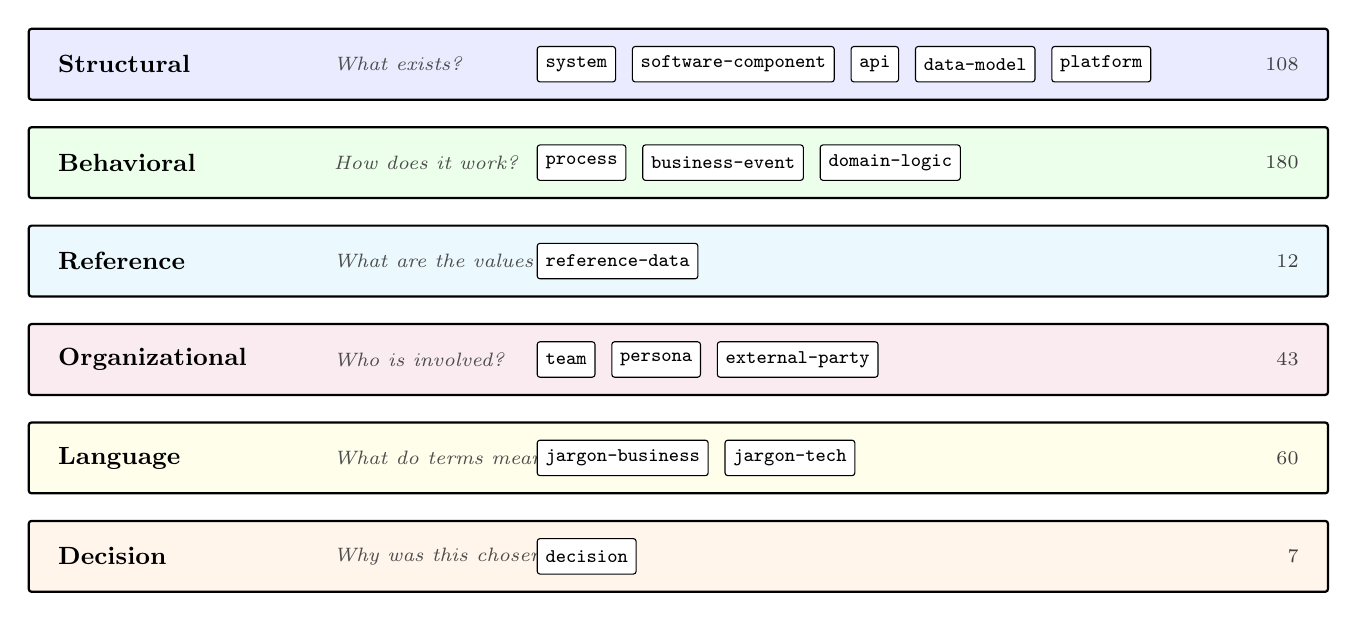
\begin{tikzpicture}[
  layer/.style={draw, thick, minimum width=16.5cm, minimum height=0.9cm, rounded corners=1pt},
  typebox/.style={draw, fill=white, font=\scriptsize\ttfamily, minimum height=0.45cm, rounded corners=1pt, inner sep=3pt},
  lbl/.style={font=\small\bfseries, anchor=west},
  qlbl/.style={font=\scriptsize\itshape, text=gray!60!black, anchor=west},
  cnt/.style={font=\scriptsize, text=gray!50!black, anchor=east},
]

\def\rowsep{1.25}
\def\typestart{-1.8}
\def\typegap{0.2cm}

% --- Structural ---
\node[layer, fill=blue!8] at (0,0) {};
\node[lbl] at (-8.0,0) {Structural};
\node[qlbl] at (-4.5,0) {What exists?};
\node[typebox, anchor=west] (s1) at (\typestart,0) {system};
\node[typebox, right=\typegap of s1] (s2) {software-component};
\node[typebox, right=\typegap of s2] (s3) {api};
\node[typebox, right=\typegap of s3] (s4) {data-model};
\node[typebox, right=\typegap of s4] (s5) {platform};
\node[cnt] at (8.0,0) {108};

% --- Behavioral ---
\node[layer, fill=green!8] at (0,-\rowsep) {};
\node[lbl] at (-8.0,-\rowsep) {Behavioral};
\node[qlbl] at (-4.5,-\rowsep) {How does it work?};
\node[typebox, anchor=west] (b1) at (\typestart,-\rowsep) {process};
\node[typebox, right=\typegap of b1] (b2) {business-event};
\node[typebox, right=\typegap of b2] (b3) {domain-logic};
\node[cnt] at (8.0,-\rowsep) {180};

% --- Reference ---
\node[layer, fill=cyan!8] at (0,-2*\rowsep) {};
\node[lbl] at (-8.0,-2*\rowsep) {Reference};
\node[qlbl] at (-4.5,-2*\rowsep) {What are the values?};
\node[typebox, anchor=west] (r1) at (\typestart,-2*\rowsep) {reference-data};
\node[cnt] at (8.0,-2*\rowsep) {12};

% --- Organizational ---
\node[layer, fill=purple!8] at (0,-3*\rowsep) {};
\node[lbl] at (-8.0,-3*\rowsep) {Organizational};
\node[qlbl] at (-4.5,-3*\rowsep) {Who is involved?};
\node[typebox, anchor=west] (o1) at (\typestart,-3*\rowsep) {team};
\node[typebox, right=\typegap of o1] (o2) {persona};
\node[typebox, right=\typegap of o2] (o3) {external-party};
\node[cnt] at (8.0,-3*\rowsep) {43};

% --- Language ---
\node[layer, fill=yellow!8] at (0,-4*\rowsep) {};
\node[lbl] at (-8.0,-4*\rowsep) {Language};
\node[qlbl] at (-4.5,-4*\rowsep) {What do terms mean?};
\node[typebox, anchor=west] (l1) at (\typestart,-4*\rowsep) {jargon-business};
\node[typebox, right=\typegap of l1] (l2) {jargon-tech};
\node[cnt] at (8.0,-4*\rowsep) {60};

% --- Decision ---
\node[layer, fill=orange!8] at (0,-5*\rowsep) {};
\node[lbl] at (-8.0,-5*\rowsep) {Decision};
\node[qlbl] at (-4.5,-5*\rowsep) {Why was this chosen?};
\node[typebox, anchor=west] (d1) at (\typestart,-5*\rowsep) {decision};
\node[cnt] at (8.0,-5*\rowsep) {7};

\end{tikzpicture}
\caption{The typed, layered knowledge base meta-model showing the 15 entity types instantiated in our healthcare claims KB (counts at right). The meta-model defines 18 types total; 3 additional types (data-product, capability, offering) are defined but not populated in this domain. DCR exploits this structure for intent classification, graph traversal, and gap detection.}
\label{fig:ontology}
\end{figure*}

% =============================================================================
% 4. DCR ARCHITECTURE
% =============================================================================
\section{DCR Pipeline Architecture}
\label{sec:pipeline}

DCR processes each query through seven sequential stages (Figure~\ref{fig:pipeline}). Stages~1--5 handle retrieval and ranking; Stage~6 synthesizes an answer; Stage~7 detects knowledge base gaps. All stages except Stage~6 are deterministic given the same knowledge base state.

\begin{figure}[t]
\centering
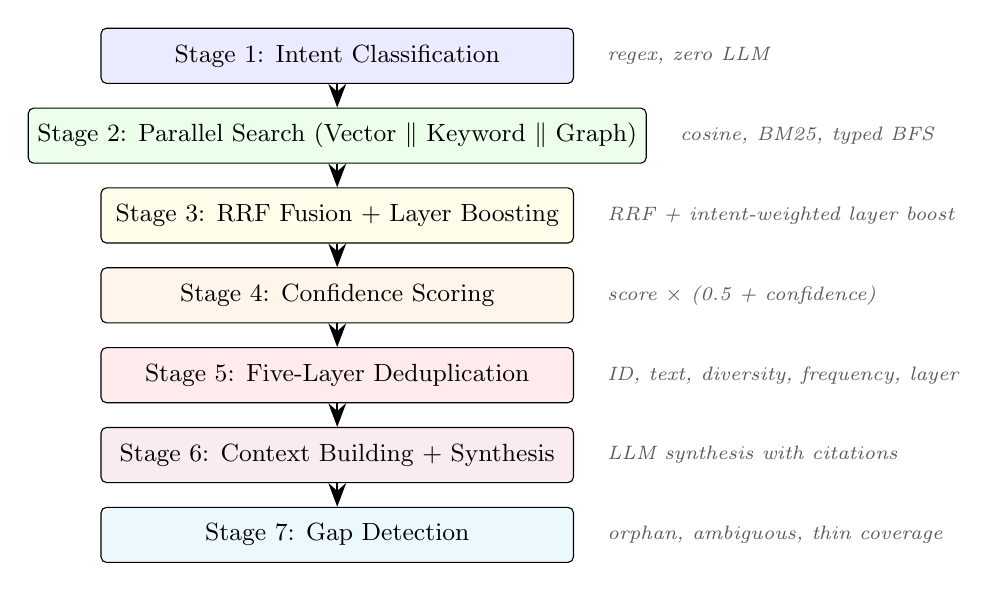
\begin{tikzpicture}[
  stage/.style={draw, rounded corners=2pt, minimum width=6cm, minimum height=0.7cm, font=\small, align=center},
  arrow/.style={-{Stealth[length=3mm]}, thick},
  note/.style={font=\scriptsize\itshape, text=gray!70!black}
]
\node[stage, fill=blue!8] (s1) {Stage 1: Intent Classification};
\node[stage, fill=green!8, below=0.3cm of s1] (s2) {Stage 2: Parallel Search (Vector $\parallel$ Keyword $\parallel$ Graph)};
\node[stage, fill=yellow!8, below=0.3cm of s2] (s3) {Stage 3: RRF Fusion + Layer Boosting};
\node[stage, fill=orange!8, below=0.3cm of s3] (s4) {Stage 4: Confidence Scoring};
\node[stage, fill=red!8, below=0.3cm of s4] (s5) {Stage 5: Five-Layer Deduplication};
\node[stage, fill=purple!8, below=0.3cm of s5] (s6) {Stage 6: Context Building + Synthesis};
\node[stage, fill=cyan!8, below=0.3cm of s6] (s7) {Stage 7: Gap Detection};

\draw[arrow] (s1) -- (s2);
\draw[arrow] (s2) -- (s3);
\draw[arrow] (s3) -- (s4);
\draw[arrow] (s4) -- (s5);
\draw[arrow] (s5) -- (s6);
\draw[arrow] (s6) -- (s7);

\node[note, right=0.3cm of s1] {regex, zero LLM};
\node[note, right=0.3cm of s2] {cosine, BM25, typed BFS};
\node[note, right=0.3cm of s3] {RRF + intent-weighted layer boost};
\node[note, right=0.3cm of s4] {score $\times$ (0.5 + confidence)};
\node[note, right=0.3cm of s5] {ID, text, diversity, frequency, layer};
\node[note, right=0.3cm of s6] {LLM synthesis with citations};
\node[note, right=0.3cm of s7] {orphan, ambiguous, thin coverage};
\end{tikzpicture}
\caption{The seven-stage DCR pipeline. Stages 1--5 handle retrieval; Stage 6 synthesizes an answer; Stage 7 detects knowledge base gaps. All stages except Stage 6 are deterministic.}
\label{fig:pipeline}
\end{figure}

\subsection{Stage 1: Intent Classification}

Intent classification determines which entity types and knowledge layers are most relevant to the query. DCR uses a zero-LLM approach: regex pattern matching against the query text to assign weights to eight fixed, hand-designed intent categories (process, ownership, entity, relationship, temporal, diagnostic, listing, comparison). These categories were derived from manual analysis of 200+ enterprise support questions across three domains during prior work on the DDC methodology~\citep{navakoti2026ddc}. Each intent maps to a weight vector over entity types and knowledge layers. For example, a process query increases weights for \textit{process}, \textit{business-event}, and \textit{domain-logic} entity types and boosts the \textit{behavioral} knowledge layer.

\subsection{Stage 2: Parallel Search}

Three search strategies run concurrently:

\begin{itemize}[nosep]
  \item \textbf{Vector search.} The query is embedded and compared against entity embeddings using cosine similarity. Returns the top-$K$ candidates ($K = 81$ for this knowledge base, approximately 20\% of entity count).
  \item \textbf{Keyword search.} BM25-style scoring against entity names and body text. Returns the same $K$ candidates.
  \item \textbf{Graph search.} Breadth-first traversal from the top vector results, following typed relationship edges. Edge types are filtered based on query intent: a process query follows \texttt{triggers}, \texttt{depends\_on}, and \texttt{implements} edges but not \texttt{owned\_by}. Maximum depth is 3 hops.
\end{itemize}

\subsection{Stage 3: RRF Fusion with Layer Boosting}

Reciprocal Rank Fusion~\citep{cormack2009rrf} merges the three candidate lists. The fused RRF score is blended with the original cosine similarity: $s = 0.7 \times s_{\text{RRF}} + 0.3 \times s_{\text{cosine}}$. Both components are normalized to $[0, 1]$: RRF scores are inherently bounded (the maximum score for the rank-1 entity is $\frac{3}{1+k}$ across 3 lists, normalized by this maximum), and cosine similarities on unit-normalized embeddings fall in $[0, 1]$. Layer priority boosting then adjusts scores based on the intent-derived layer weights from Stage~1.

\subsection{Stage 4: Confidence Scoring}

Each entity carries a confidence score (0.0--1.0) reflecting its curation quality---description completeness, relationship density, and source document coverage. Confidence scoring adjusts the retrieval score: $s' = s \times (0.5 + c)$, where $c$ is the entity's confidence. The 0.5 floor ensures that even minimally documented entities retain half their retrieval score. Additional boosts account for relationship density ($\log(1 + \text{edge\_count})$) and source document count.

\subsection{Stage 5: Five-Layer Deduplication}

Deduplication applies five sequential filters: (1)~exact entity ID dedup, (2)~text similarity dedup (cosine $> 0.85$ on body text), (3)~type diversity enforcement (limits entities per type based on intent), (4)~inverse frequency weighting (deprioritizes ubiquitous entities), and (5)~layer diversity enforcement (ensures representation across knowledge layers).

\subsection{Stage 6: Context Building and Synthesis}

Retrieved entities are assembled into \emph{typed context blocks}---structured text segments that include each entity's full body text, type label, layer assignment, confidence score, and relationship summary (Figure~\ref{fig:context-block}). These blocks are concatenated into the LLM's context window. An LLM synthesizes an answer with entity-level citations and self-scores the answer as ANSWERABLE, PARTIAL, or NOT\_ANSWERABLE, which we map to CLEAN, INCOMPLETE, and MISSING respectively (see Section~\ref{sec:scoring}).

\begin{figure}[t]
\begin{lstlisting}
--- ENTITY: Eligibility Service ---
Type: system | Layer: structural | Confidence: 0.92
Related: Claims Gateway (depends_on),
         Rules Engine (depends_on),
         Eligibility Check API (exposes)

The Eligibility Service verifies member coverage
for claims submitted to Clearview Health Plans.
It provides point-in-time eligibility lookups via
the /eligibility/{memberId}/asof/{date} endpoint,
supporting retroactive checks up to 2 years.

During adjudication, the Rules Engine queries
accumulators through this service. Soft reservations
prevent concurrent claims from double-applying
against benefit limits. Each reservation tracks
claim ID, amount, accumulator type, and timestamp.

The September 2022 outage caused 18,000-claim
backlog when Eligibility Service timeouts triggered
503 errors in the Claims Gateway.
---
\end{lstlisting}
\caption{A typed context block as assembled in Stage~6 for a well-connected entity. Each block contains the entity's full body text alongside typed metadata (type, layer, confidence, relationships). The distinction between this rich context and metadata-only context (name, type, description) is central to the synthesis bottleneck finding (Section~\ref{sec:discussion}).}
\label{fig:context-block}
\end{figure}

\begin{figure}[t]
\begin{lstlisting}
--- ENTITY: After-Hours Routing ---
Type: domain-logic | Layer: behavioral | Conf: 0.41
Related: (none)

After-hours routing applies when claims arrive
outside the 7am-7pm CT processing window.
Priority claims route to the overnight queue;
standard claims hold until next business day.
---

GAP SIGNAL [orphan_entity]: "After-Hours Routing"
  retrieved with score 0.78 but has zero typed
  relationships to other retrieved entities.
  Suggested action: document which system owns
  this logic and which process triggers it.
\end{lstlisting}
\caption{A sparse context block triggering an orphan gap signal. Contrast with Figure~\ref{fig:context-block}: low confidence (0.41), no relationships, and a short body. Stage~7 identifies this as a curation target---the knowledge exists but is disconnected from the entity graph.}
\label{fig:gap-example}
\end{figure}

\subsection{Stage 7: Gap Detection}

Gap detection examines the retrieval trace to identify two primary types of knowledge base deficiencies:

\begin{itemize}[nosep]
  \item \textbf{Orphan entities.} Entities retrieved with high relevance but no typed relationships to other retrieved entities---indicating missing relationship documentation.
  \item \textbf{Ambiguous entities.} Pairs of retrieved entities with high name or content similarity but different types---indicating potential duplicates or unclear type boundaries.
\end{itemize}

A third gap type, \textbf{thin coverage}, fires when the retrieval set meets the top-$K$ threshold but content density is low and the answer is classified as MISSING. In our evaluation (Section~\ref{sec:gaps}), this type did not fire due to the near-zero MISSING rate.

Gap detection is downstream of retrieval and independent of answer quality. Its output is a structured list of gap signals, each with a type, severity, and description. These signals target knowledge base curators, not end users.

% =============================================================================
% 5. EXPERIMENTAL SETUP
% =============================================================================
\section{Experimental Setup}
\label{sec:setup}

\subsection{Knowledge Base}

We use a synthetic healthcare claims processing domain: Clearview Health Plans, a fictional regional health insurer. The meta-model defines 18 entity types across 6 layers; this knowledge base instantiates 15 of those types with 410 entities (Table~\ref{tab:kb-stats}). Three types (data-product, capability, offering) are defined in the schema but not populated in this domain.

The Behavioral layer dominates the distribution (180/410, 44\%) because healthcare claims processing is a process-heavy domain: adjudication workflows, event-driven routing, and business rules generate more documentable entities than the structural systems that execute them.

The knowledge base was constructed in three stages. First, 148 synthetic source documents were generated describing the domain's systems, processes, APIs, data models, teams, and terminology. Second, an automated extraction pipeline (Claude Sonnet with a typed meta-model schema) processed each document to identify entities, assign types and layers, extract relationships, and generate confidence scores based on description completeness, relationship density, and source document coverage. Third, extracted entities underwent manual curation review: deduplication, relationship validation, and quality assessment. The pipeline and source documents are included in the repository.

\begin{table}[t]
\centering
\caption{Knowledge base composition by layer.}
\label{tab:kb-stats}
\begin{tabular}{@{}lcc@{}}
\toprule
Layer & Types (populated) & Entity Count \\
\midrule
Structural & 5 & 108 \\
Behavioral & 3 & 180 \\
Reference & 1 & 12 \\
Organizational & 3 & 43 \\
Language & 2 & 60 \\
Decision & 1 & 7 \\
\midrule
\textbf{Total} & \textbf{15} & \textbf{410} \\
\bottomrule
\end{tabular}
\end{table}

\subsection{Evaluation Questions}

We generated evaluation questions using Claude Sonnet from seed context consisting of 10 representative entity descriptions sampled across all 6 layers. The generation prompt requested questions that a domain practitioner might ask, spanning both single-system lookups and cross-system integration queries. From an initial pool of 73 generated questions, we deduplicated to 50 using a dual threshold: Jaccard similarity $> 0.55$ on question tokens and entity overlap $> 0.7$ on extracted entity references. Because questions were generated from entity descriptions in the same knowledge base the pipeline queries, the evaluation vocabulary aligns with entity names and terminology---this represents a best-case scenario for retrieval and may inflate absolute CLEAN rates compared to questions from real users who use less precise terminology. We note this as a limitation (Section~\ref{sec:limitations}). Questions span two categories based on their layer hints: 28 \emph{cross-cutting} questions requiring synthesis across multiple entity types and layers (no layer hint assigned), and 22 \emph{single-layer} questions addressable from entities within a single knowledge layer.

\subsection{Conditions}
\label{sec:conditions}

We evaluate 9 retrieval conditions: 3 baselines and 6 ablation variants.

\paragraph{Baselines.}
\begin{itemize}[nosep]
  \item \textbf{Naive vector.} Cosine similarity only. No keyword search, no graph traversal, no fusion, no typed stages.
  \item \textbf{Vanilla RAG.} Vector search plus keyword search with simple score averaging. No typed traversal, no confidence scoring, no dedup beyond ID matching.
  \item \textbf{DCR.} Full seven-stage pipeline.
\end{itemize}

\paragraph{Ablation.} Each variant removes one stage from the full DCR pipeline:
\begin{itemize}[nosep]
  \item \textbf{full\_dcr}: control condition (identical pipeline to DCR, run as a separate trial batch to quantify inter-batch scoring variance).
  \item \textbf{no\_intent}: Stage~1 removed; flat, uniform layer weights.
  \item \textbf{no\_graph}: Stage~2 graph traversal removed; vector + keyword search only.
  \item \textbf{no\_layer\_boost}: Stage~3 layer priority boosting removed from fusion.
  \item \textbf{no\_confidence}: Stage~4 confidence scoring removed.
  \item \textbf{no\_dedup}: Stage~5 multi-layer dedup replaced with simple ID dedup.
\end{itemize}

\subsection{Scoring}
\label{sec:scoring}

Each retrieved context is passed to Claude Sonnet\footnote{Model: \texttt{claude-sonnet-4-20250514} (Anthropic API, May 2025).} for synthesis and self-scoring in a single LLM call. The model generates an answer with entity citations and self-scores as ANSWERABLE, PARTIAL, or NOT\_ANSWERABLE. We map these to a three-class DDC taxonomy:

\begin{itemize}[nosep]
  \item \textbf{CLEAN}: the knowledge base fully addresses the question.
  \item \textbf{INCOMPLETE}: the knowledge base partially addresses the question but key information is missing.
  \item \textbf{MISSING}: the knowledge base does not contain enough information to answer.
\end{itemize}

The same model is used for both synthesis and scoring. While this introduces a potential self-enhancement bias~\citep{zheng2023judging}, we mitigate it in three ways: (1)~multi-trial averaging reduces single-run variance, (2)~an independent cross-model check re-scores answers without retrieval context (Section~\ref{sec:judge}), and (3)~we report relative comparisons across conditions---any systematic bias affects all conditions equally.

Each condition is run 3 independent times (separate LLM scoring runs on identical retrieval results) to characterize scoring variance. Total evaluations: 50 questions $\times$ 9 conditions $\times$ 3 trials = 1,350.

\subsection{Latency}
\label{sec:latency}

Table~\ref{tab:latency} reports per-query latency, measured from checkpoint timestamps. Retrieval stages (1--5 and 7) complete in under 300ms across all conditions; LLM synthesis (Stage~6) dominates at 10--12s median. The retrieval overhead of DCR's typed stages over naive vector search is approximately 60ms ($\sim$30\% relative increase), negligible compared to synthesis latency. All experiments ran on a single machine (Apple M3 Max, 36GB) with local vector indices and the Anthropic API for synthesis.

\begin{table}[t]
\centering
\caption{Per-query latency (median across all trials, in milliseconds).}
\label{tab:latency}
\begin{tabular}{@{}lccc@{}}
\toprule
Condition & Retrieval & Synthesis & Total \\
\midrule
Naive Vector & 199 & 10{,}329 & 10{,}524 \\
Vanilla RAG & 218 & 9{,}393 & 9{,}619 \\
DCR & 255 & 11{,}294 & 11{,}568 \\
\bottomrule
\end{tabular}
\end{table}

\subsection{Judge Consistency}
\label{sec:judge}

We assessed cross-model reliability by re-scoring 30 (question, answer) pairs using GPT-4o as an independent judge: 15 from DCR and 15 from vanilla RAG, each proportionally stratified by actual DDC class distribution. Cross-model agreement with Claude's original scoring was 80.0\% (24/30). Cohen's $\kappa = 0.47$ (moderate agreement). The relatively low kappa despite 80\% raw agreement reflects the skewed class distribution: with $>$70\% of answers classified as CLEAN, chance agreement is high, which mechanically depresses $\kappa$. All 6 disagreements were one-directional \emph{promotions} (INCOMPLETE~$\to$~CLEAN), with 3 per condition---affecting both conditions equally and preserving the relative comparison. GPT-4o confirmed the DCR quality advantage: 14/15 DCR answers scored CLEAN vs.\ 12/15 for vanilla RAG.

% =============================================================================
% 6. RESULTS
% =============================================================================
\section{Results}
\label{sec:results}

\subsection{Baseline Comparison}

Table~\ref{tab:baselines} and Figure~\ref{fig:baselines} show the baseline comparison. DCR achieves 76.0\% CLEAN, a 16.7 percentage point improvement over vanilla RAG (59.3\%) and a 6.7pp improvement over naive vector search (69.3\%).

\begin{table}[t]
\centering
\caption{Baseline comparison (mean $\pm$ SD across 3 trials, $n = 50$ questions per trial).}
\label{tab:baselines}
\begin{tabular}{@{}lccc@{}}
\toprule
Condition & CLEAN (\%) & INCOMPLETE (\%) & MISSING (\%) \\
\midrule
Naive Vector & $69.3 \pm 1.2$ & $30.7 \pm 1.2$ & $0.0 \pm 0.0$ \\
Vanilla RAG & $59.3 \pm 3.1$ & $38.7 \pm 3.1$ & $2.0 \pm 0.0$ \\
DCR (ours) & $\mathbf{76.0 \pm 0.0}$ & $24.0 \pm 0.0$ & $0.0 \pm 0.0$ \\
\bottomrule
\end{tabular}
\end{table}

\begin{figure}[t]
\centering
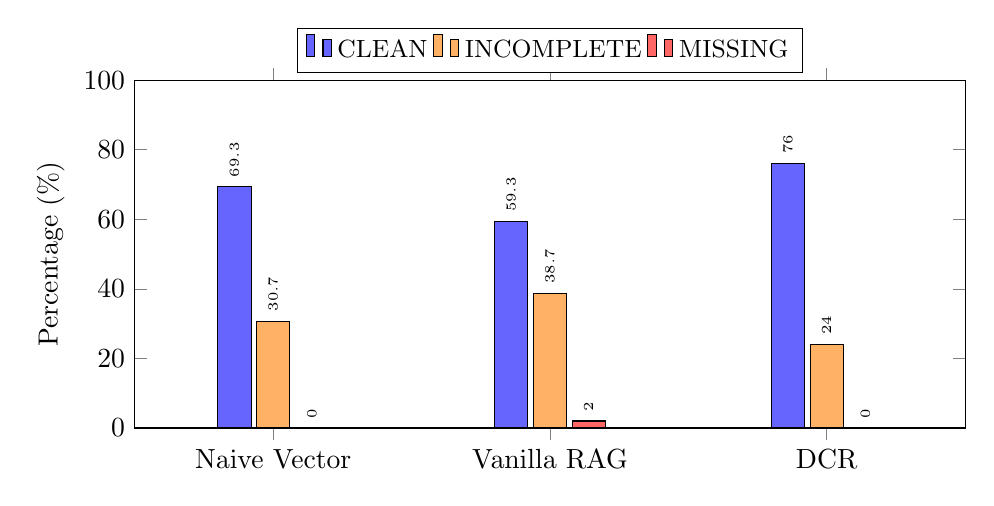
\begin{tikzpicture}
\begin{axis}[
    ybar,
    bar width=12pt,
    width=\columnwidth,
    height=6cm,
    ylabel={Percentage (\%)},
    symbolic x coords={Naive Vector, Vanilla RAG, DCR},
    xtick=data,
    ymin=0, ymax=100,
    legend style={at={(0.5,1.02)}, anchor=south, legend columns=3, font=\small},
    nodes near coords style={font=\tiny, rotate=90, anchor=west},
    enlarge x limits=0.25,
    every node near coords/.append style={xshift=0pt},
]
\addplot[fill=blue!60, nodes near coords] coordinates {(Naive Vector,69.3) (Vanilla RAG,59.3) (DCR,76.0)};
\addplot[fill=orange!60, nodes near coords] coordinates {(Naive Vector,30.7) (Vanilla RAG,38.7) (DCR,24.0)};
\addplot[fill=red!60, nodes near coords] coordinates {(Naive Vector,0.0) (Vanilla RAG,2.0) (DCR,0.0)};
\legend{CLEAN, INCOMPLETE, MISSING}
\end{axis}
\end{tikzpicture}
\caption{Baseline comparison of DDC class distributions. DCR achieves the highest CLEAN rate (76.0\%) and zero MISSING. Naive vector (69.3\%) outperforms vanilla RAG (59.3\%) due to score-averaging noise in the latter.}
\label{fig:baselines}
\end{figure}

\subsection{Statistical Tests}

The CLEAN rate difference between DCR and vanilla RAG is statistically significant. We constructed a $2 \times 2$ contingency table (CLEAN vs.\ non-CLEAN $\times$ DCR vs.\ vanilla RAG, pooling all 150 observations per condition): DCR produced 114 CLEAN and 36 non-CLEAN; vanilla RAG produced 89 CLEAN and 61 non-CLEAN. Chi-square test: $\chi^2 = 8.78$, $df = 1$, $p = 0.003$.

For overall quality, we encoded DDC classes as ordinal values (CLEAN~$= 3$, INCOMPLETE~$= 2$, MISSING~$= 1$; treated as an ordinal scale, not interval) and applied the Mann-Whitney U test: $U = 13{,}179$, $p = 0.0016$, significant at $\alpha = 0.01$. The Kruskal-Wallis test across all three baselines is also significant: $H = 10.35$, $p = 0.006$.

MISSING rates show a floor effect: 8 of 9 conditions achieve 0.0\% MISSING, with only vanilla RAG producing any MISSING answers (3/150, 2.0\%). A Fisher exact test comparing DCR (0/150) to vanilla RAG (3/150) is not significant: $p = 0.248$. On this well-curated, dense knowledge base, catastrophic retrieval failure is rare regardless of retrieval method.

\subsection{Naive Vector Outperforms Vanilla RAG}

An unexpected result: naive vector search (69.3\% CLEAN) substantially outperforms vanilla RAG (59.3\%), a 10.0pp gap. This inversion occurs because vanilla RAG uses simple score averaging to combine vector and keyword search results. On a knowledge base where entity descriptions are rich, typed, and well-curated, keyword search surfaces entities that match query terms but are contextually less relevant. Averaging the keyword score with the vector score dilutes the signal from strong semantic matches. Naive vector search, using only cosine similarity, avoids this noise.

This finding underscores that the \emph{typed ontology}---entity types, curated descriptions, semantic layers, and relationships---is the primary driver of retrieval quality, not the retrieval pipeline. When the underlying content is well-structured, even the simplest retrieval method produces good results. Critically, this does not mean keyword search is inherently harmful on typed KBs---DCR also uses keyword search but avoids signal degradation by combining results through Reciprocal Rank Fusion (which respects rank ordering) rather than raw score averaging. DCR's advantage over naive vector (+6.7pp) comes from this structured fusion, combined with graph traversal and deduplication that the simpler method cannot perform.

\subsection{Stratification: Cross-Cutting vs.\ Single-Layer}

Table~\ref{tab:stratified} shows results stratified by question type, pooled across all 3 trials.

\begin{table}[t]
\centering
\caption{Stratified results: cross-cutting vs.\ single-layer questions (pooled across 3 trials).}
\label{tab:stratified}
\begin{tabular}{@{}llcccc@{}}
\toprule
Condition & Stratum & $N$ & CLEAN (\%) & INC (\%) & MISS (\%) \\
\midrule
\multirow{2}{*}{Naive Vector} & Cross-cutting & 84 & 72.6 & 27.4 & 0.0 \\
& Single-layer & 66 & 65.2 & 34.8 & 0.0 \\
\addlinespace
\multirow{2}{*}{Vanilla RAG} & Cross-cutting & 84 & 59.5 & 36.9 & 3.6 \\
& Single-layer & 66 & 59.1 & 40.9 & 0.0 \\
\addlinespace
\multirow{2}{*}{DCR} & Cross-cutting & 84 & 76.2 & 23.8 & 0.0 \\
& Single-layer & 66 & 75.8 & 24.2 & 0.0 \\
\bottomrule
\end{tabular}
\end{table}

DCR achieves balanced performance across both question types (76.2\% vs.\ 75.8\%), showing that the typed pipeline handles cross-cutting questions as well as single-layer ones. Vanilla RAG shows uniformly lower performance across both strata (59.5\% vs.\ 59.1\%). Naive vector shows a 7.4pp gap between strata (72.6\% vs.\ 65.2\%), suggesting that cosine-only retrieval is less effective at gathering related entities for single-layer questions where structural navigation helps.

\subsection{Per-Question Stability}
\label{sec:stability}

We measure per-question stability as the percentage of questions that receive the same DDC classification across all 3 trials. Table~\ref{tab:stability} reports stability for all conditions.

\begin{table}[t]
\centering
\caption{Per-question stability across 3 trials (percentage of questions with identical classification in all trials).}
\label{tab:stability}
\begin{tabular}{@{}lc@{}}
\toprule
Condition & Stability (\%) \\
\midrule
DCR & \textbf{96} \\
no\_intent & 94 \\
Vanilla RAG & 92 \\
Naive Vector & 90 \\
full\_dcr & 90 \\
no\_layer\_boost & 90 \\
no\_dedup & 88 \\
no\_confidence & 84 \\
no\_graph & 82 \\
\bottomrule
\end{tabular}
\end{table}

DCR achieves the highest stability (96\%), meaning that 48 of 50 questions receive the same classification in every trial. This contradicts an intuition that more complex pipelines should produce more variable results. Instead, the structured retrieval produces consistent context windows, which in turn produce consistent LLM scoring. The least stable condition is no\_graph (82\%), suggesting that removing graph traversal introduces context variability.

% =============================================================================
% 7. ABLATION ANALYSIS
% =============================================================================
\section{Ablation Analysis}
\label{sec:ablation}

\subsection{Stage Contributions}

Table~\ref{tab:ablation} and Figure~\ref{fig:ablation} show the effect of removing individual pipeline stages. The full\_dcr condition serves as the ablation control; differences between full\_dcr (72.0\%) and the DCR baseline (76.0\%) reflect inter-batch scoring variance---the same pipeline scored in a separate trial batch. This 4.0pp gap is within the range of LLM scoring variance observed across conditions (SD up to 3.5pp for no\_confidence) and does not indicate a systematic difference. All ablation comparisons use full\_dcr as the reference to ensure within-batch fairness. Note that no\_intent at 76.0\% matching the DCR baseline is coincidental; the relevant comparison is no\_intent vs.\ full\_dcr ($+4.0$pp, $p = 0.43$).

\begin{table}[t]
\centering
\caption{Ablation study (mean $\pm$ SD across 3 trials, $n = 50$). $\Delta$CLEAN is relative to full\_dcr.}
\label{tab:ablation}
\begin{tabular}{@{}lcccc@{}}
\toprule
Condition & CLEAN (\%) & INC (\%) & MISS (\%) & $\Delta$CLEAN \\
\midrule
full\_dcr & $72.0 \pm 2.0$ & $28.0 \pm 2.0$ & $0.0 \pm 0.0$ & --- \\
\addlinespace
no\_intent & $76.0 \pm 2.0$ & $24.0 \pm 2.0$ & $0.0 \pm 0.0$ & $+4.0$ \\
no\_graph & $68.0 \pm 2.0$ & $32.0 \pm 2.0$ & $0.0 \pm 0.0$ & $-4.0$ \\
no\_layer\_boost & $74.0 \pm 2.0$ & $26.0 \pm 2.0$ & $0.0 \pm 0.0$ & $+2.0$ \\
no\_confidence & $72.0 \pm 3.5$ & $28.0 \pm 3.5$ & $0.0 \pm 0.0$ & $0.0$ \\
no\_dedup & $74.0 \pm 0.0$ & $26.0 \pm 0.0$ & $0.0 \pm 0.0$ & $+2.0$ \\
\bottomrule
\end{tabular}
\end{table}

\begin{figure}[t]
\centering
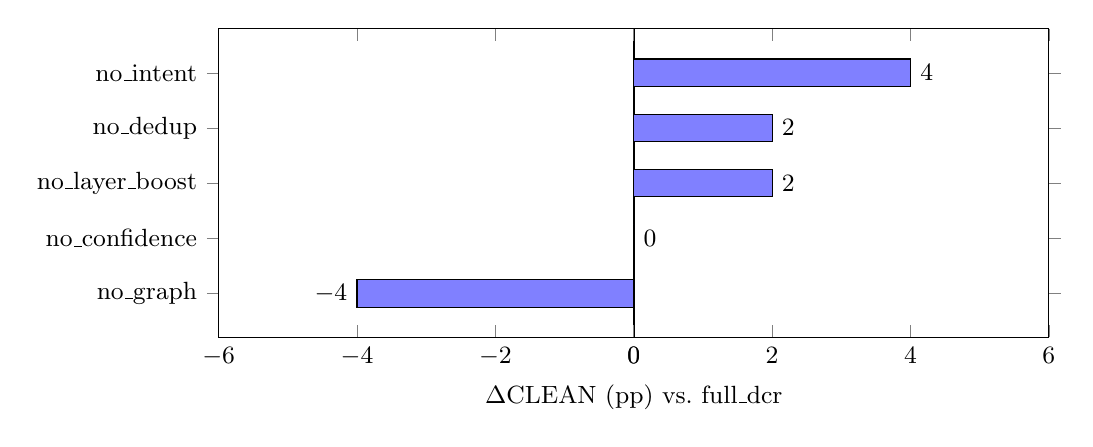
\begin{tikzpicture}
\begin{axis}[
    xbar,
    bar width=10pt,
    width=\columnwidth,
    height=5.5cm,
    xlabel={$\Delta$CLEAN (pp) vs.\ full\_dcr},
    symbolic y coords={no\_graph, no\_confidence, no\_layer\_boost, no\_dedup, no\_intent},
    ytick=data,
    xmin=-6, xmax=6,
    nodes near coords,
    nodes near coords style={font=\small},
    enlarge y limits=0.2,
    extra x ticks={0},
    extra x tick style={grid=major, grid style={black, thick}},
    tick label style={font=\small},
    label style={font=\small},
]
\addplot[fill=blue!50] coordinates {(4.0,no\_intent) (2.0,no\_dedup) (2.0,no\_layer\_boost) (0.0,no\_confidence) (-4.0,no\_graph)};
\end{axis}
\end{tikzpicture}
\caption{Ablation: change in CLEAN rate when each stage is removed, relative to the full\_dcr control. No individual stage produces a statistically significant effect (all $p > 0.43$). Graph traversal shows the largest negative impact ($-4.0$pp); intent classification shows the largest positive impact ($+4.0$pp).}
\label{fig:ablation}
\end{figure}

\subsection{No Individual Stage Is Statistically Significant}

Pairwise Mann-Whitney U tests comparing each ablation condition against full\_dcr yield no significant results (Table~\ref{tab:ablation-pvals}). The largest effect is $\pm 4.0$pp (no\_intent and no\_graph), both with $p > 0.43$.

\begin{table}[t]
\centering
\caption{Ablation pairwise tests vs.\ full\_dcr (Mann-Whitney U, $n = 150$ per condition).}
\label{tab:ablation-pvals}
\begin{tabular}{@{}lcc@{}}
\toprule
Condition & $\Delta$CLEAN (pp) & $p$-value \\
\midrule
no\_intent & $+4.0$ & 0.431 \\
no\_graph & $-4.0$ & 0.451 \\
no\_layer\_boost & $+2.0$ & 0.698 \\
no\_confidence & $0.0$ & 1.000 \\
no\_dedup & $+2.0$ & 0.698 \\
\bottomrule
\end{tabular}
\end{table}

This result does not mean the stages are useless. The typed pipeline as a whole produces a 16.7pp improvement over vanilla RAG. Rather, the ablation reveals that on a dense, well-curated knowledge base (410 entities, high average confidence), no single stage is the bottleneck. The stages contribute collectively through small, additive effects that fall below the detection threshold of per-stage ablation at this sample size.

\subsection{Directional Observations}

While not statistically significant, three directional patterns emerge:

\begin{enumerate}[nosep]
  \item \textbf{Graph traversal helps.} Removing graph search produces the largest negative effect ($-4.0$pp) and the lowest stability (82\%). Graph-retrieved entities provide structurally connected context that vector similarity alone misses.
  \item \textbf{Intent classification may hurt on dense KBs.} Removing intent classification produces the largest \emph{positive} effect ($+4.0$pp). On a 410-entity knowledge base where most types are well-represented, intent-based layer weighting may overly restrict the candidate pool. This pattern is consistent with the hypothesis that typed stages are density-dependent, though we have not tested this at other scales (see Section~\ref{sec:limitations}).
  \item \textbf{Confidence scoring is neutral.} Removing confidence scoring produces zero change in CLEAN rate. On a knowledge base where most entities have high confidence scores (a consequence of thorough DDC curation), confidence weighting provides no discriminative signal.
\end{enumerate}

% =============================================================================
% 8. GAP DETECTION
% =============================================================================
\section{Gap Detection as Retrieval Observability}
\label{sec:gaps}

\subsection{Gap Signal Distribution}

Table~\ref{tab:gaps} summarizes gap detection behavior across conditions. Gap detection only fires in DCR-family conditions (those that include typed graph traversal and relationship analysis). Baseline conditions (naive vector and vanilla RAG) produce zero gap signals because they lack the structural analysis required to identify orphan entities and ambiguous types.

\begin{table}[t]
\centering
\caption{Gap detection summary (averaged across 3 trials).}
\label{tab:gaps}
\begin{tabular}{@{}lccc@{}}
\toprule
Condition & Trigger Rate (\%) & Signals/Trial & Types \\
\midrule
DCR & 80.0 & 62 & 37 ambig., 25 orphan \\
full\_dcr & 80.0 & 62 & 37 ambig., 25 orphan \\
no\_intent & 64.0 & 39 & 17 ambig., 22 orphan \\
no\_graph & 80.0 & 68 & 49 ambig., 19 orphan \\
no\_layer\_boost & 74.0 & 49 & 20 ambig., 29 orphan \\
no\_confidence & 82.0 & 62 & 36 ambig., 26 orphan \\
no\_dedup & 80.0 & 62 & 37 ambig., 25 orphan \\
\addlinespace
Naive Vector & 0.0 & 0 & --- \\
Vanilla RAG & 0.0 & 0 & --- \\
\bottomrule
\end{tabular}
\end{table}

\subsection{Thin Coverage and the Floor Effect}

The original design of gap detection included a \emph{thin coverage} signal intended to predict MISSING answers: when the retrieval set meets the top-$K$ threshold but content density is low and the answer is MISSING. In our evaluation, zero thin-coverage gaps were detected across all 1,350 evaluations. This is a direct consequence of the MISSING floor effect: with only 3 MISSING answers total (all in vanilla RAG, which does not produce gap signals), the trigger condition for thin coverage was never satisfied.

This does not invalidate the thin-coverage mechanism---it indicates that the current knowledge base is too well-curated and dense for this signal to fire. On sparser or less-curated knowledge bases, thin coverage may prove valuable. We note this as a limitation requiring evaluation on knowledge bases with higher MISSING rates.

\subsection{Gap Detection as Curation Feedback}

The consistent 80\% trigger rate and 62 signals per evaluation, \emph{independent of answer quality}, position gap detection as an observability mechanism rather than a confidence metric. Every query surfaces structural information about the knowledge base:

\begin{itemize}[nosep]
  \item \textbf{Orphan entities} (25 per evaluation): entities retrieved with high relevance but no relationships to co-retrieved entities, indicating missing documentation of how these entities connect to the broader domain.
  \item \textbf{Ambiguous entities} (37 per evaluation): pairs of retrieved entities with high similarity but different types, indicating potential duplicates or unclear type boundaries that curators should resolve.
\end{itemize}

These signals feed directly back into the DDC curation cycle~\citep{navakoti2026ddc}: each gap signal identifies a specific curation action (document a relationship, resolve a type ambiguity) that improves the knowledge base for future queries.

% =============================================================================
% 9. DISCUSSION
% =============================================================================
\section{Discussion}
\label{sec:discussion}

\subsection{The Synthesis Bottleneck}

RAG system design implicitly assumes that retrieval quality is the primary lever for answer quality. Our results, combined with an inadvertent ablation during development, suggest a different bottleneck: \emph{the richness of content that reaches the synthesis LLM matters more than how it was selected}.

During development, a bug in the synthesis stage caused only entity metadata (name, type, description, relationship IDs) to be passed to the LLM, rather than the full entity body text shown in Figure~\ref{fig:context-block}. The same pipeline, the same retrieval stages, and the same questions produced radically different results depending on whether the LLM received metadata-only or full-text context. This inadvertent ablation of \emph{context content richness} produced larger effect sizes than any retrieval stage ablation---evidence for a principle we term the \emph{synthesis bottleneck}: context composition quality sets the ceiling on answer quality, and no retrieval improvement can compensate for shallow content.

This principle generalizes beyond our specific implementation. In any RAG system, even perfect retrieval produces poor answers if the context window contains shallow, poorly-curated, or metadata-only content. The implication for practitioners is that investments in knowledge base curation quality---the depth and richness of entity descriptions---may yield larger returns than investments in retrieval pipeline sophistication. Our typed context blocks (Figure~\ref{fig:context-block}) are designed to maximize the richness of the synthesis input, which is why DCR's architecture treats curation quality (Stage~4) and context composition (Stage~5--6) as first-class pipeline concerns rather than afterthoughts.

\subsection{Typed Ontology vs.\ Typed Retrieval}

Our results reveal a clean separation between two sources of value:

\begin{enumerate}[nosep]
  \item \textbf{The typed ontology} (entity types, layers, relationships, curated descriptions) makes \emph{every} retrieval method better. Naive vector achieves 69.3\% CLEAN on this well-structured knowledge base---higher than vanilla RAG at 59.3\%.
  \item \textbf{The typed retrieval stages} (intent classification, graph traversal, layer boosting, confidence scoring, multi-layer dedup) provide an additional 6.7pp lift from naive vector to DCR (76.0\%). This lift is real but modest compared to the ontology's contribution.
\end{enumerate}

This distinction is important for practitioners deciding where to invest effort. Building a well-typed, well-curated knowledge base using a methodology like DDC appears to be the higher-leverage investment. Adding typed retrieval stages on top provides diminishing but still meaningful returns.

\subsection{Implications for Knowledge Base Design}

The near-zero MISSING rate across 8 of 9 conditions suggests that on a 410-entity knowledge base with thorough curation, the primary quality challenge is INCOMPLETE answers (24--39\% across conditions), not MISSING ones. The remaining quality gap lies in entities that are documented but not documented \emph{enough}---a curation depth problem rather than a coverage problem.

We note that INCOMPLETE is the largest quality class after CLEAN in every condition, yet our evaluation does not characterize it further. Our data does not reveal whether INCOMPLETE concentrates in cross-cutting questions (which require synthesis across layers) or in specific entity types, nor whether it correlates with entity confidence scores. The stratified results (Table~\ref{tab:stratified}) show similar INCOMPLETE rates across cross-cutting and single-layer strata for DCR (23.8\% vs.\ 24.2\%), suggesting that question complexity is not the primary driver, but the 50-question sample is too small for definitive conclusions. Understanding what makes an answer INCOMPLETE rather than CLEAN---whether it is missing relationships, shallow entity descriptions, or absent supporting entities---is an important direction for future analysis and would directly inform curation priorities.

This aligns with the DDC methodology's incremental curation approach: as cycles of failure analysis identify gaps and curators fill them, the knowledge base moves from MISSING-dominated (early) to INCOMPLETE-dominated (mature) to CLEAN-dominated (well-curated). Our results characterize the INCOMPLETE-to-CLEAN transition boundary, where retrieval strategy provides diminishing returns and curation depth becomes the bottleneck.

\subsection{Full DCR vs.\ DCR Baseline Variance}

The full\_dcr control condition (72.0\% CLEAN) differs from the DCR baseline (76.0\% CLEAN) by 4.0pp, despite using identical pipelines. This gap reflects inter-batch LLM scoring variance---the same (question, context) pairs scored in different trial batches can produce different classifications. This variance is inherent to LLM-as-judge evaluation and should be factored into the interpretation of all results. Our ablation comparisons use full\_dcr (not the DCR baseline) as the reference to ensure fair within-batch comparison.

% =============================================================================
% 10. LIMITATIONS AND REPRODUCIBILITY
% =============================================================================
\section{Limitations and Reproducibility}
\label{sec:limitations}

\subsection{Limitations}

\begin{itemize}[nosep]
  \item \textbf{Single knowledge base.} All experiments use one synthetic domain. Generalization to other domains, knowledge base sizes, and entity type distributions is not established.
  \item \textbf{Synthetic data.} The knowledge base was generated and curated, not extracted from a production environment. Production knowledge bases may have different quality distributions, particularly lower average confidence scores.
  \item \textbf{LLM judge with self-scoring.} The same model generates and scores answers, introducing potential self-enhancement bias~\citep{zheng2023judging}. Our GPT-4o cross-model check ($n = 30$, 80\% agreement, $\kappa = 0.47$) shows identical promotion patterns across conditions, suggesting the bias does not distort relative comparisons. However, absolute DDC class rates may differ under human evaluation.
  \item \textbf{No $K$ sensitivity analysis.} The top-$K$ retrieval threshold ($K = 81$, approximately 20\% of entity count) was not ablated. Different $K$ values may affect both baseline and DCR results.
  \item \textbf{Small question set.} 50 questions provide adequate power for the CLEAN comparison ($p = 0.003$) but limit per-question-type analysis and prevent detection of small ablation effects. The non-significant ablation results may reflect insufficient statistical power rather than true null effects.
  \item \textbf{LLM-generated questions.} Evaluation questions were generated by an LLM from seed context rather than drawn from real user queries, potentially biasing the question distribution.
  \item \textbf{MISSING floor effect.} With 0\% MISSING in 8 of 9 conditions, we cannot assess DCR's impact on catastrophic failure reduction. This question requires evaluation on sparser knowledge bases with higher MISSING rates.
  \item \textbf{Density hypothesis untested.} The observation that intent classification may hurt on dense knowledge bases is a directional finding at one scale point, not a confirmed relationship. Validation at multiple knowledge base sizes is needed.
\end{itemize}

\subsection{Reproducibility}

We release the pipeline implementation, evaluation questions, knowledge base, and all 1,350 checkpoint files (one per evaluation, containing the question, retrieved entities, synthesized answer, DDC classification, gap signals, and retrieval trace metadata). Trial-level and aggregate statistics are computed from these checkpoints. An earlier version of this experiment contained a synthesis pipeline bug that passed only entity metadata to the LLM rather than full body text; the results in this paper are from the corrected pipeline. Both versions of the code and their respective results are preserved in the repository for transparency.\footnote{\url{https://github.com/ea-toolkit/dcr-paper}}

% =============================================================================
% 11. CONCLUSION
% =============================================================================
\section{Conclusion}
\label{sec:conclusion}

We presented Domain-Constrained Retrieval, a seven-stage pipeline for typed, layered knowledge bases. On a 410-entity healthcare claims knowledge base, DCR achieves 76.0\% CLEAN answers---a 16.7 percentage point improvement over vanilla RAG ($p = 0.003$)---with 96\% per-question stability across trials.

Our most striking finding is that naive vector search (69.3\%) outperforms vanilla RAG (59.3\%) on this typed knowledge base, revealing that the \emph{typed ontology}---well-curated entity descriptions, explicit type assignments, and semantic layer organization---is the primary quality driver. The typed retrieval stages provide an additional 6.7pp lift, meaningful but secondary to the ontology's contribution.

Stage-by-stage ablation reveals no individually significant stage contributions on this dense knowledge base (all $p > 0.43$), though graph traversal shows a consistent directional positive effect ($-4.0$pp when removed) and is the only stage whose removal also degrades stability (82\% vs.\ 96\%). Intent classification shows a directional negative effect, consistent with the hypothesis that typed stages are density-dependent, though validation at other scales is needed. Gap detection fires on 80\% of questions, producing 62 curation signals per evaluation independently of answer quality---an observability mechanism that feeds back into the knowledge curation cycle.

The synthesis bottleneck---the finding that context content richness dominates retrieval strategy as a quality determinant---has practical implications: investments in knowledge base curation depth may yield larger returns than investments in retrieval pipeline sophistication. Our results suggest that for practitioners working with typed knowledge bases, building a well-curated ontology is the higher-leverage first step.

Future work includes (1)~validating the density hypothesis by evaluating DCR on structurally different knowledge bases of varying size and density---partitioning the current 410-entity KB would test size but not structural diversity, so evaluation on additional domains (e.g., fintech operations, supply chain logistics) is needed, (2)~scaling to 200+ questions with human-calibrated scoring rubrics, (3)~evaluating on production knowledge bases with higher MISSING rates to test the thin-coverage gap detection mechanism, and (4)~multi-model evaluation to reduce dependence on single-judge scoring. In practice, our results suggest teams should first invest in building a typed ontology with rich entity descriptions, then layer typed retrieval on top---the ontology is the foundation, the pipeline is the refinement.

% =============================================================================
% REFERENCES
% =============================================================================
\begin{thebibliography}{99}

\bibitem[Asai et~al.(2024)]{asai2024selfrag}
A.~Asai, Z.~Wu, Y.~Wang, A.~Sil, and H.~Hajishirzi.
\newblock Self-{RAG}: Learning to retrieve, generate, and critique through self-reflection.
\newblock In \emph{ICLR}, 2024.

\bibitem[Bordes et~al.(2013)]{bordes2013transe}
A.~Bordes, N.~Usunier, A.~Garcia-Duran, J.~Weston, and O.~Yakhnenko.
\newblock Translating embeddings for modeling multi-relational data.
\newblock In \emph{NeurIPS}, 2013.

\bibitem[Chen et~al.(2024)]{chen2024bge}
J.~Chen, S.~Xiao, P.~Zhang, K.~Luo, D.~Lian, and Z.~Liu.
\newblock {BGE} {M3}-Embedding: Multi-lingual, multi-functionality, multi-granularity text embeddings through self-knowledge distillation.
\newblock \emph{arXiv preprint arXiv:2402.03216}, 2024.

\bibitem[Cormack et~al.(2009)]{cormack2009rrf}
G.~V.~Cormack, C.~L.~A.~Clarke, and S.~B{\"u}ttcher.
\newblock Reciprocal rank fusion outperforms {Condorcet} and individual rank learning methods.
\newblock In \emph{SIGIR}, 2009.

\bibitem[Edge et~al.(2024)]{edge2024graphrag}
D.~Edge, H.~Trinh, N.~Cheng, J.~Bradley, A.~Chao, A.~Mody, S.~Truitt, and J.~Larson.
\newblock From local to global: A graph {RAG} approach to query-focused summarization.
\newblock \emph{arXiv preprint arXiv:2404.16130}, 2024.

\bibitem[Hu et~al.(2024)]{hu2024grag}
Z.~Hu, Z.~Xu, G.~Qi, and K.~Wang.
\newblock {GRAG}: Graph retrieval-augmented generation.
\newblock \emph{arXiv preprint arXiv:2405.16506}, 2024.

\bibitem[Lewis et~al.(2020)]{lewis2020rag}
P.~Lewis, E.~Perez, A.~Piktus, F.~Petroni, V.~Karpukhin, N.~Goyal, H.~K{\"u}ttler, M.~Lewis, W.-t.~Yih, T.~Rockt{\"a}schel, S.~Riedel, and D.~Kiela.
\newblock Retrieval-augmented generation for knowledge-intensive {NLP} tasks.
\newblock In \emph{NeurIPS}, 2020.

\bibitem[Liu et~al.(2025)]{liu2025consjudge}
S.~Liu, X.~Li, Z.~Liu, Y.~Yan, C.~Yang, Z.~Zeng, Z.~Liu, M.~Sun, and G.~Yu.
\newblock Judge as a judge: Improving the evaluation of retrieval-augmented generation through the judge-consistency of large language models.
\newblock In \emph{Findings of ACL}, pages 5788--5807, 2025.

\bibitem[Navakoti and Navakoti(2026)]{navakoti2026ddc}
R.~Navakoti and S.~Navakoti.
\newblock Demand-driven context: A methodology for building enterprise knowledge bases through agent failure.
\newblock \emph{arXiv preprint arXiv:2603.14057}, 2026.

\bibitem[Press et~al.(2023)]{press2023selfask}
O.~Press, M.~Zhang, S.~Min, L.~Schmidt, N.~A.~Smith, and M.~Lewis.
\newblock Measuring and narrowing the compositionality gap in language models.
\newblock In \emph{Findings of EMNLP}, 2023.

\bibitem[Rajpurkar et~al.(2018)]{rajpurkar2018squad}
P.~Rajpurkar, R.~Jia, and P.~Liang.
\newblock Know what you don't know: Unanswerable questions for {SQuAD}.
\newblock In \emph{ACL}, 2018.

\bibitem[Sarmah et~al.(2024)]{sarmah2024hybridrag}
B.~Sarmah, B.~Hall, R.~Rao, S.~Patel, S.~Pasupuleti, and M.~Kulkarni.
\newblock {HybridRAG}: Integrating knowledge graphs and vector retrieval augmented generation for efficient information extraction.
\newblock \emph{arXiv preprint arXiv:2408.04948}, 2024.

\bibitem[Shankar et~al.(2024)]{shankar2024validates}
S.~Shankar, J.~Zamfirescu-Pereira, B.~Hartmann, A.~Parameswaran, and I.~Arawjo.
\newblock Who validates the validators? {A}ligning {LLM}-assisted evaluation of {LLM} outputs with human preferences.
\newblock In \emph{UIST}, 2024.

\bibitem[Zheng et~al.(2023)]{zheng2023judging}
L.~Zheng, W.-L.~Chiang, Y.~Sheng, S.~Zhuang, Z.~Wu, Y.~Zhuang, Z.~Lin, Z.~Li, D.~Li, E.~P.~Xing, H.~Zhang, J.~E.~Gonzalez, and I.~Stoica.
\newblock Judging {LLM}-as-a-judge with {MT-Bench} and {Chatbot Arena}.
\newblock In \emph{NeurIPS}, 2023.

\end{thebibliography}

\end{document}
